\documentclass[a4paper, 12pt]{article}

\usepackage[T2A]{fontenc}
\usepackage[utf8]{inputenc}
\usepackage[english,russian]{babel} %локализация
\usepackage{graphicx}%Вставка картинок правильная
\usepackage{float}%"Плавающие" картинки
\usepackage{wrapfig}%Обтекание фигур (таблиц, картинок и прочего)
\usepackage{fancybox,fancyhdr} %колонтитулы
\usepackage{amsmath, amsfonts, amssymb, amsthm, mathtools} %математика
\usepackage[left=2cm,right=2cm,
    top=1.5cm,bottom=1.5cm,bindingoffset=0cm]{geometry}
%\usepackage[12pt]{extsizes} % размер шрифта

%\documentclass[a4paper]{article}
\usepackage[14pt]{extsizes}
\usepackage[T2A]{fontenc}
\usepackage[utf8]{inputenc}
\usepackage[russian]{babel}
\usepackage{setspace,amsmath}
\usepackage{graphicx}
\usepackage{epigraph}
\usepackage{csquotes}
\usepackage[unicode, pdftex, hidelinks]{hyperref}
\usepackage{amssymb}
\usepackage{caption}
\usepackage{amsthm}
\usepackage{float}
\usepackage{wrapfig}
\usepackage{multirow}
\usepackage[left=15mm, top=10mm, right=10mm, bottom=15mm, nohead, footskip=10mm]{geometry}
%\pagestyle{fancy}
\newtheorem*{theorem}{\sc{Theorem}}
\newtheorem*{definition}{\sc{Definition}}
\newtheorem*{proposition}{\sc{Proposition}}
\newtheorem*{corollary}{\sc{Corollary}}
\newtheorem*{claim}{\sc{Claim}}
\newtheorem*{properties}{\sc{Properties}}
\newtheorem*{remark}{\sc{Remark}}
\DeclareMathOperator{\N}{\mathbb{N}}
\DeclareMathOperator{\Z}{\mathbb{Z}}
\DeclareMathOperator{\Q}{\mathbb{Q}}
\DeclareMathOperator{\R}{\mathbb{R}}
\RequirePackage{caption}
\DeclareCaptionLabelSeparator{d}{}
\captionsetup{justification=centering,labelsep=d}


%% Перенос знаков в формулах (по Львовскому)
\newcommand*{\hm}[1]{#1\nobreak\discretionary{}
{\hbox{$\mathsurround=0pt #1$}}{}}


\author{Вехов В. В.}

\title{Волчок Томсона (китайский волчок) \\ Вопрос по выбору}

\date{2024}

\begin{document}
\maketitle
\\\
\\\
\\\
\center{
\includegraphics[scale=0.2]{logo.png}}
\newpage

\tableofcontents{}
\newpage

\section{Введение}
В данной работе расмотрим физику движения гироскопа в случае волчка Томпсона, тажке известного как китайский волчок или тип-тoп.
Исследование китайского волчка является интереснейшей областью изучения динамики
вращательного движения и гироскопических эффектов. \newline
Волчок Томсона — волчок, обладающий свойством переворачиваться в процессе вращения. Этот волчок отличается от своих собратьев тем, что в процессе вращения его центр масс поднимается. Благодаря специальной форме и распределению массы по телу волчка может возникнуть усложненное вращение: через некоторое время после начала вращения из положения ножкой кверху волчок переходит в стадию вращения на боку ножкой горизонтально, а затем скачкообразно переворачивается на ножку с поднятием центра тяжести и начинает вращаться, касаясь плоскости вершиной ножки с сохранением направления вращения.


\section{Цель работы}
исследовать физику гироскопа и вращения волчка Томпсона.

\subsection{Гироскоп}

\subsubsection{Общая информация}

Гироскоп —  прибор для обнаружения вращения. В широком смысле это быстро вращающееся тело, ось вращения которого может менять свое расположение в пространстве. Простейший пример гироскопа — волчок.\newline
При этом скорость вращения гироскопа значительно превышает скорость поворота оси его вращения. Основное свойство гироскопа — способность сохранять в пространстве неизменное направление оси вращения при отсутствии воздействия на него моментов внешних сил и эффективно сопротивляться действию внешних моментов сил. Это свойство в значительной степени определяется величиной угловой скорости собственного вращения гироскопа.\newline
Наиболее широкое употребление у симметричных гироскопов, волчок Томпсона как раз относится к ним.
\begin{figure}	\center{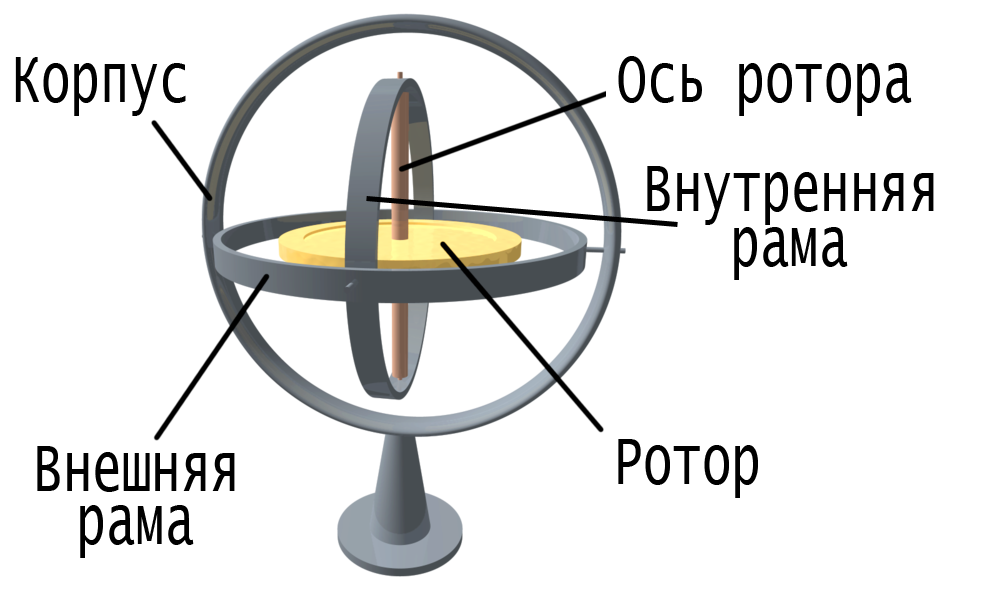
\includegraphics[scale=0.2]{hirosc.png}}
 \end{figure}

\subsubsection{Фомула гироскопа}

Все явления обусловленные быстрым вращением гироскопа называтся гироскопическими. Они нашли широкое научно-техническое применение.\newline
Согласно теореме Эйлера движение гироскопа с неподвижной точкой опоры можно представить как вращение вокруг мгновенной оси, проходящей через эту точку. обозгачим вектор угловой скорости, проходящей через эту точку, момент импульса гироскопа относительно точки О. Поскольку для симметричных тел, вращающихся вокруг главной оси, момент импульса равен произведению момента инерции тела на
угловую скорость его вращения, то для гироскопа:
\begin{equation}
		L = I \omega
\end{equation}
Момент инерции I
зависит от массы и от ее распределения относительно оси вращения.
Величина вектора L определяет точность работы гироскопических приборов.
Чем она больше, тем устойчивее и точнее работают эти приборы
Движение гироскопа, как твердого тела, определяется уравнением
динамики вращательного движения: скорость изменения момента импульса
вращающегося тела равняется суммарному моменту внешних сил,
действующих на него:
\begin{equation}
		\label{Torque}
		\frac{d \vec{L}}{dt} = \vec{M}
\end{equation}
Где M - сумма моментов внешних сил.
\center{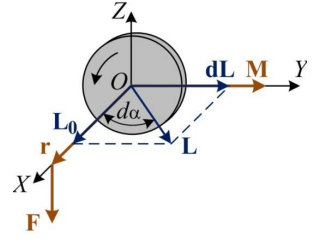
\includegraphics[scale=0.7]{hiro.png}}

Применим основное уравнение
динамики вращательного движения. В результате действия силы F в
течение времени dt начальный момент импульса L0 получит приращение
dL = Mdt
, где М – момент силы F относительно точки О. Новый момент
импульса
L = L0 + dL
отклонится относительно первоначального
направления на некоторый угол da в горизонтальной плоскости (произойдет
поворот вектора момента импульса вокруг оси Z). Поскольку при больших
угловых скоростях вектор L направлен вдоль оси гироскопа, то вместе с L
на угол da повернется и сама ось.\newline
В ходе прецессии ось гироскопа поворачивается вокруг вертикальной
оси Z, проходящей через точку опоры О, с угловой скоростью прецессии
Характерной особенностью прецессии является ее безынерционность
(четвертое свойство свободного гироскопа): прецессионное движение
существует в течение времени действия внешней силы и мгновенно
прекращается с ее исчезновением.

\subsection{Волчок Томсона}

\subsubsection{Общая информация}
Теперь перейдем к рассмотрению волчков. Волчок Томсона необычный волчок: в  отличие от остальных он в результате прецессии встает на свою ножку, поднимая тем самым свой центр тяжести и его потенциальная энергия увеличивется.\newline
Для начала рассмотрим обычный вращающийся дискообразный волчок. В начале вращения, когда угловая скорость велика, его ось практически вертикальна. Затем угловая скорость вращения под действием сил трения в точке опоры и о воздух уменьшается, и волчок начинает прецессировать вокруг вертикальной оси, описывая коническую поверхность с вершиной в точке опоры. На волчок действуют сила тяжести, сила реакции опоры (эти силы создают момент силы, изменяющий момент импульса волчка по направлению). Следует заметить, что прецессия оси существовала и в самом начале из-за неизбежного точка, который сообщается при раскручивании. \newline
Кроме этих сил есть еще сила трения, которая создает момент, направленный к вертикале, поэтому благодаря трению ось волчка стремится занять вертикальное положение. В этом легко убедитяся, запустив волчок под наклоном. Момент силы трения зависит от выбора оси, относительно которой он расчитывается, поэтому будем его считать относительно центра инерции.
\\\
\center{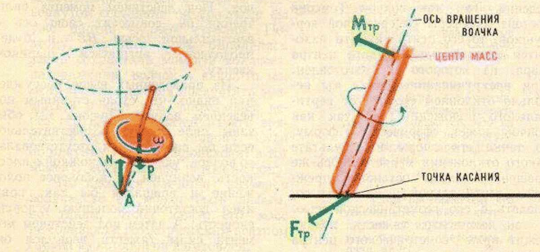
\includegraphics[scale=0.62]{волчок.png}}
\\\
\\\
Итак, существуют два момента сил: тяжести, реакции опоры и силы трения.
Вернемся теперь к волчку Томсона и попробуем объяснить его поведение.

\subsubsection{Динамика}

Так как волчок Томсона состоит из сферы сос срезанной верхушкой, то его центр тяжести находится ниже геометрического центра шара.
При раскручивании волчка мы невольно отклоняем его ось от вертикальной оси. Из-за того, что он имеет сферическую форму, то точка его опоры в результате такого отклонения меняется.Ось вращения будет оставаться прежней и волчок будет прецесссировать вокруг вертикали. Центр тяжести уже не будет лежать на оси вращения (в точке O') и будет вращеся вокруг вертикальной оси. Момент силы трения будет изменять вектор момента импульса по направлению и модулю, тем самым переворачивая волчок (как показано на рисунке). При малых углах момент силы трения относительно центр инерции стремится вернуть ось волчка к вертикали, но при больших углах отклонения момент силы трения изменяет момент импульса и старается его опрокинуть из-за низкого расположения центр инерции.
\begin{equation}
		\frac{d \vec{L}}{dt} = \vec{M_{tr}}
\end{equation}
\begin{equation}
		\vec{M_{tr}} = [\vec{r}, \vec{F_{tr}}]
\end{equation}
\\\
\\\
При вращении с большой угловой скоростью центр тяжести будет подниматься точно так же, как поднимается шарик на нити, еслт нить раскручивать (как показано на рисунке) в следствие центробежной силы.
\center{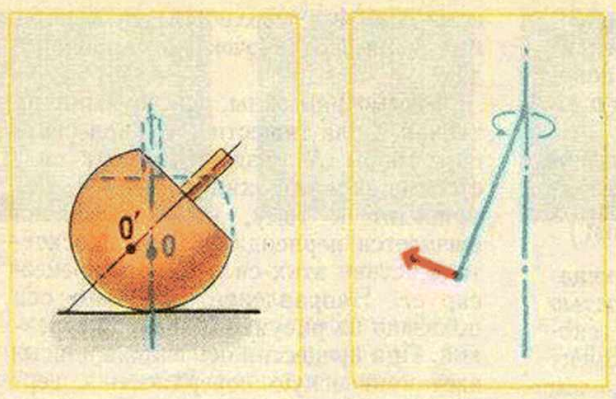
\includegraphics[scale=0.45]{волчок2.png}}
\newline
\\\
Волчок не задерживается в боковом пололжении (в этот момент останавливет собственное вращение), а по инерции проскакивает его, касаясь нижней ножкой плосоксти. Как только это произойдет, точка опоры перескочит из точки А в точку B и будет прецессировать вокруг оси BB' и будет вращаться шариком кверху.
Из приведенных выше рассуждений видно, что этому поведению волчка мы обязаны силе трения. Благодаря ей волчок вскакивает на ножку в момент её касания.

\center{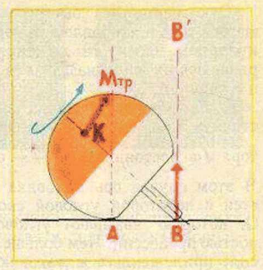
\includegraphics[scale=0.55]{волчок3.png} 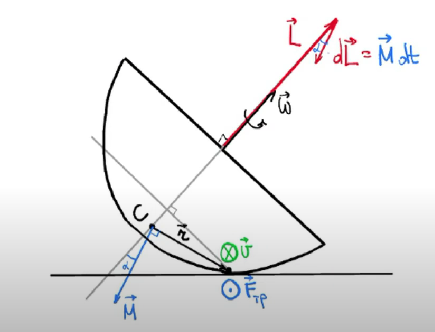
\includegraphics[scale=0.55]{волчок4.png}
\\\
\\\
Что касается расчетов размеров волчка, то он может быть любым, но таким, чтобы центр его масс не совпадал с геометрическим центром
сферы, из которой он изготовлен.
\\\
В процессе исследования я заметил, что волчок сохраняет направление вращения вокруг вертикали в начале и в конце, хотя кажется, что волчок должен крутиться в другую сторону, когда он встал на ножку. Секрет данного явления в том, что во время, когда волочок крутится на боку (на экваторе) он останавливет собвтсвенное врщение и начинает раскручиваться в другую сторону. Все это происходит по закону сохранения момента количества движения. Поэтому волчок должен вращаться в одну и ту же сторону.

\subsubsection{Зависимость от трения}
Как известно, необычному поведению волчка мы обязаны силе трения, которая вначале создает момент сил, опрокидывющий волчок, а затем момент, который поднимет волчок на ножку.
Момент силы трения волчка изменяет его момент импульса, до тех пор, пока
волчок не переворачивается на ножку.
Интересным фактом является то, что кинетическая энергия зависит от угловой скорости квадратично, а потому уменьшение кинетической энергии происходит быстрее, чем диссипация энергии от трения, оставшаяся энергии идёт на изменение потенциальной энергии – на подъём центра тяжести волчка.
зависимость такая: чем выше
шероховатость, тем более низкую угловую скорость необходимо задать для начала прецессии волчка Томпсона. На основании этого можно сказать, что на весь процесс поднятия центра тяжести влияют два основных фактора. Изменение кинетической энергии, квадратично зависящей от скорости и потери энергии на трение
при возникновении опрокидывающего момента, которые зависят от скорости
предположительно линейно.\newline
Переоворот волчка зависит еще от радиуса пятна касания поверхности. Чем оно больше тем меньше энергии требуется для переворота.


\section{Выводы}
Исследовав механику вращения китйского волчка и динамику прецессии, моджно сделать вывод, что главным фактором изменения потенциальной энергии является поднятие центра тяжести, которое происходит за счёт падения кинетической энергии при возникновении момента от трени. \newline
Резултат зависит от коэффициента трения поверхности, от начальной вращательной энергии волчка, от расположения центра масс.

Если все требования будут выполнены, волочок перевернется и будет вращатся на своей ножке.

\section{Используемая литература}
1. Л.Д.Ландау Е.М.Лифшиц "Теоретическая физика. Механика"\newline
2. Википедия — свободная энциклопедия\newline
3. "ИЗУЧЕНИЕ СВОЙСТВ МЕХАНИЧЕСКОГО
ГИРОСКОПА С ТРЕМЯ СТЕПЕНЯМИ
СВОБОДЫ" ТПУ \newline
4. Д.В.Сивухин "Общий курс физики." \newline
5. C.А.Кривошлыков "Механика вращающегося волчка" \newline
6. Адуенко А.А., Амелькин Н.И. О предельных движениях волчка с внутренней диссипацией в однородном
поле тяжести // Труды Московского физико-технического института. – 2013. – Т. 5, № 2(18). – С. 126-133.
\end{document}
